\section{Resumé}

Les appareils de numérisation et d'acquisition en 3D se sont aujourd'hui démocratisés. Si les techniques d'acquisition peuvent être différentes (scanner avec contact, scanner sans contact), le but est tojours d'obtenir une représentation 3D de l'objet scanné. Il existe plusieurs méthodes pour représenter un objet en 3D mais dans ce document nous nous pencherons sur les représentations par nuage de point.\\

Un nuage de point est décrit comme une suite de triplet $\{x_{i},y_{i},z_{i}\}$ qui représentent chacun un point dans $\mathbb{R}^3$. L'image \ref{fig_nuage_bunny} est une visualisation d'un de ces nuages de points. On peut remarquer que les points ne sont pas ordonnés, et que la surface n'existe pas réellement. 

\begin{figure}[H]
\centering
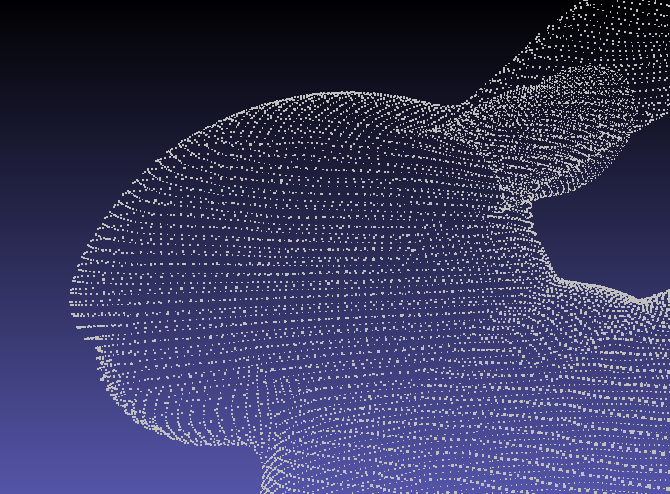
\includegraphics[width = 0.5\textwidth]{Images/Resume/nuage_bunny}
\caption{Nuage de point synthétique représentant une tête de lapin}
\label{fig_nuage_bunny}
\end{figure}

Souvent, cependant, on dispose de plusieurs nuages de points du même objet. En effet, due à la nature solide des objets, on est souvent incapable d'obtenir un nuage 3D complet d'un objet en une seule fois. Pour résoudre ce problème, on prends plusieurs nuages de points du même objet sous différents points de vue. Cependant, même si on connait la position approximative du capteur pour chaque prise de vue, les nuages de points ne seront pas exactement superposés. On est obligé de passer par une étape dite de \textit{recalage}. L'image \ref{fig_nuage_recalage} montre deux scènes identiques qui ont été prises de deux entroits différents. On remarquera une forte rotation entre les deux nuages de points.

\begin{figure}[H]
\centering
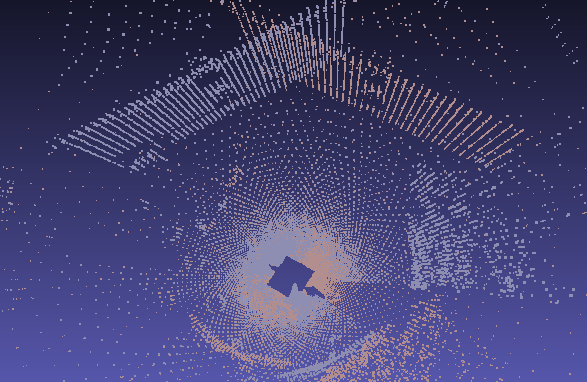
\includegraphics[width = 0.7\textwidth]{Images/Resume/nuage_recalage}
\caption{Deux nuages de points (en bleu clair et en rose) de la même scène qui n'ont pas été prises depuis le même point de vue}
\label{fig_nuage_recalage}
\end{figure}

Pour recaler ces nuages de points, il existe un certain nombre de méthodes. L'une d'elle en particulier est très souvent décrite par la littérature : l'algorithme ICP (ou Iterative Closest Point). Décrite dans \cite{bib_icp} par Besl et McKay en 1992, cet algorithme est à la fois intuitif et simple à mettre en œuvre. La première étape consiste à mettre en correspondance les points du nuage. Dans un second temps, la transformation optimale est obtenue en minimisant au sens de la méthode des moindre carrés l'énergie suivante :

\begin{equation}
E(R,t) = \sum_{i}\|b_{i}-(R*a_{i} + t)\|^{2}
\end{equation}

Dans cette énergie, $a_{i}$ et $b_{i}$ sont des triplets de coordonnées, $R$ est une matrice de rotation, t est un vecteur de translation.

Un algorithme similaire à l'ICP est appelé "Point-to-Plane" ICP. Dans ce cas, au lieu de s'intéresser à la distance entre deux points, la métrique change pour représenter la distance entre un point et le plan tangent au point de destination (cf figure \ref{fig_pointtoplane}

\begin{figure}[H]
\centering
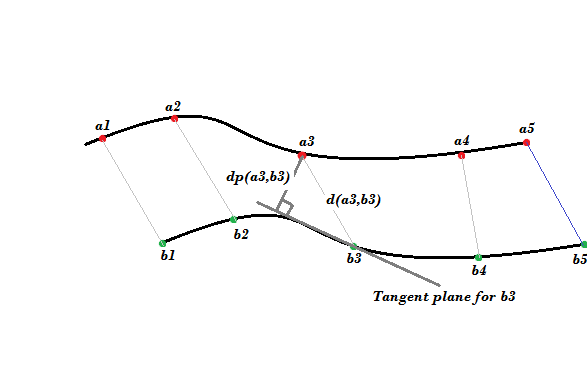
\includegraphics[width = 0.7\textwidth]{Images/Resume/icp_pointplan}
\caption{Métrique Point-to-plane (dp(a3,b3)) comparée à la métrique Point-to-point (d(a3,b3)}
\label{fig_pointtoplane}
\end{figure}

Dans le cas de l'ICP Point-to-plane, on cherche à minimiser au sens de la méthode des moindre carrés l'énergie suivante :

\begin{equation}
E(R,t) = \sum_{i} \|(b_{i}-(R*a_{i} + t)).n_{i}\|^{2}
\end{equation}	

Dans cette énergie, $a_{i}$ et $b_{i}$ sont des triplets de coordonnées, $R$ est une matrice de rotation, t est un vecteur de translation, et $n_{i}$ est la normale associée au point $b_{i}$.\\

Si dans les deux algorithmes, la minimisation de l'énergie peut être coûteuse, des implémentations très efficaces ont été mises au point. Pour l'ICP, une résolution de la minimisation de l'énergie a permis de mettre en évidence une solution analytique. Pour la version Point-to-plane, la méthode des moindre carrés non linéaires peut être linéarisée (accélérant ainsi la minimisation de l'énergie) tout en gardant une bonne approximation du résultat.
